% -*- root: main.tex -*-
%-------------------------------------------------------------------------------
\chapterimage{chapter_head_3.pdf} 

%-------------------------------------------------------------------------------
\chapter{ROS 설치 (SBC or VirtualBox)}\label{cha:ros_install_sbc}

%-------------------------------------------------------------------------------
\section{가상 머신에 ROS Indigo 설치하기}\index{가상 머신에 ROS Indigo 설치하기}

%-------------------------------------------------------------------------------
\subsection{우분투 14.04 이미지 준비}\index{우분투 14.04 이미지 준비}

ROS의 사용은 기본적으로 \textbf{섹션~\ref{sec:ROSInstallation}~\nameref{sec:ROSInstallation}(pp.\pageref{sec:ROSInstallation})} 에서와 같이 우분투를 기본 운영체제로 사용한다. 그 이외에도 윈도우즈와 OS X 등에서도 사용은 가능하나 일부 기능을 사용 못하거나 일일이 소스를 받아서 재컴파일할 필요가 있다. 그래서 이번 챕터에서는 윈도우즈에 가상 머신을 설치하여 윈도우즈 환경에서 우분투를 실행하는 가상 머신을 활용하는 방법에 대해서 다룰 예정이다. 간단히 테스트하거나 튜토리얼 정도는 이 방법으로 할 수 있을 것이다. 참고로 가상 머신은 본 챕터에서 소개하는 오픈소스 기반의 VirtualBox\footnote{\url{https://www.virtualbox.org/}} 이외에도 상용 제품인 VMware\footnote{\url{http://www.vmware.com/}}, Parallels\footnote{\url{http://www.parallels.com/}} 등이 있다. 자신에게 맞는 것을 사용하도록 하자.

이 방법은 가상 머신 사용으로 인해 2개의 운영체제가 CPU를 나누어 쓰게되어 속도면에서 매우 본래 목적인 ROS 사용에 있어서 속도면에서 지장을 준다. 필자는 가상 머신보다는 우분투만 사용하거나 혹은 윈도우즈와 멀티부팅으로 사용하기를 추천한다. 간단한 테스트 목적 및 학습 목적이라면 이 방법으로 \textbf{챕터~\ref{cha:RosPrograming}~\nameref{cha:RosPrograming}(pp.\pageref{cha:RosPrograming})} 수행에는 전혀 문제 없다.

우선, 그림\ref{fig:download_ubuntu}와 같이 \url{http://www.ubuntu.com/download/desktop/} 에서 우분투 ISO 이미지파일을 다운로드 하자. 우분투는 14.04.x LTS 로 선택하고, 자신의 컴퓨터의 사양에 따라 32bit 혹은 64bit 를 골라 다운로드 하자.

\begin{figure}[h]
\centering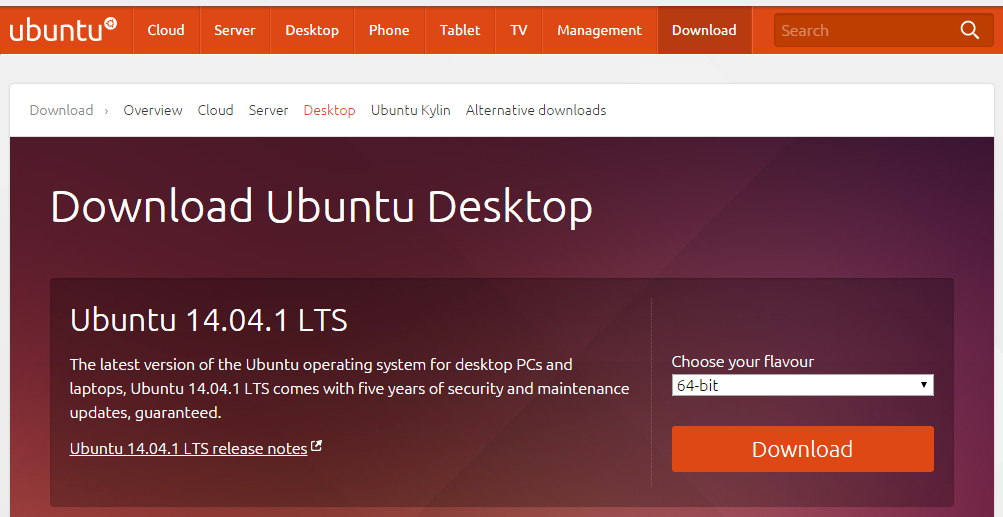
\includegraphics[width=0.5\columnwidth]{pictures/chapter3/ubuntu_web.png}
\caption{우분투 이미지 파일 다운로드}
\label{fig:download_ubuntu}
\end{figure}

%-------------------------------------------------------------------------------
\subsection{Virtualbox 설치}\index{Virtualbox 설치}

\begin{figure}[h]
\centering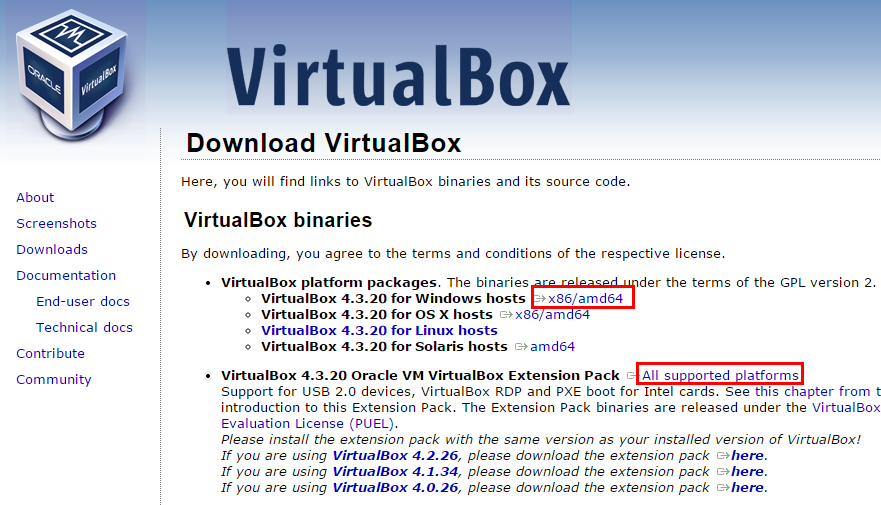
\includegraphics[width=0.7\columnwidth]{pictures/chapter3/virtual_box_web.png}
\caption{Virtual Box 다운로드}
\label{fig:download_vm}
\end{figure}

그림\ref{fig:download_vm}와 같이 VirtualBox 4.3.xx for Windows hosts 와 VirtualBox 4.3.20 Oracle VM VirtualBox Extension Pack 을 다운로드 하자. 설치 방법은 매우 간단하다. 다음의 설치 과정의 그림들을 참고해 가며 설치하도록 하자.

\begin{figure}[h]
\centering
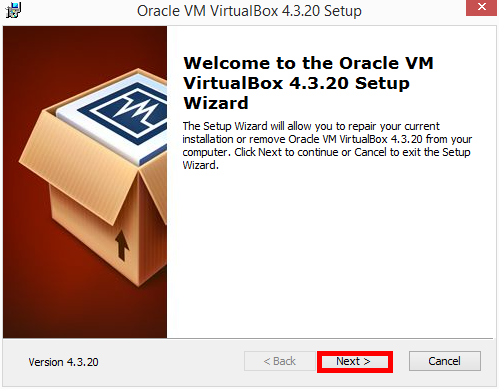
\includegraphics[width=0.42\columnwidth]{pictures/chapter3/vm1.png}
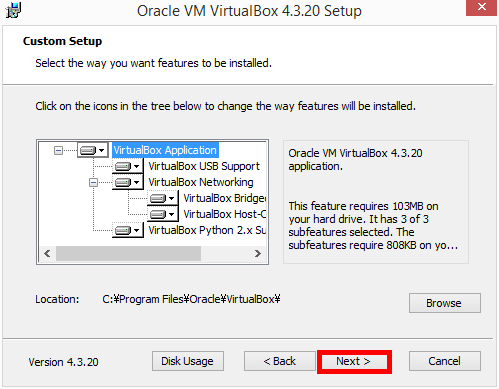
\includegraphics[width=0.42\columnwidth]{pictures/chapter3/vm2.png}
\end{figure}

\begin{figure}[h]
\centering
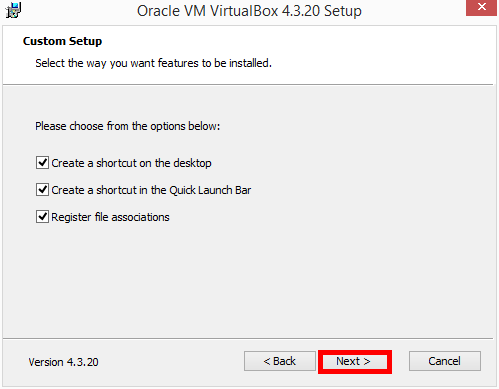
\includegraphics[width=0.42\columnwidth]{pictures/chapter3/vm3.png}
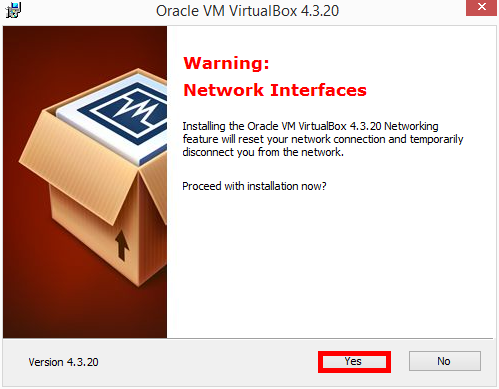
\includegraphics[width=0.42\columnwidth]{pictures/chapter3/vm4.png}
\end{figure}

\newpage

\begin{figure}[h]
\centering
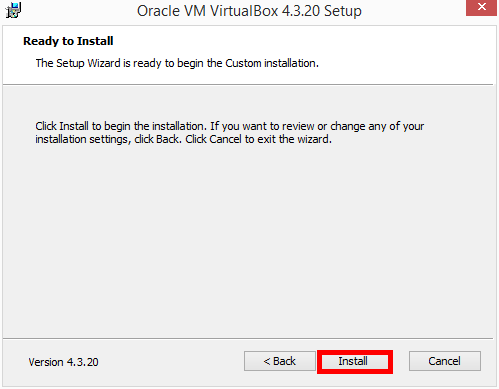
\includegraphics[width=0.49\columnwidth]{pictures/chapter3/vm5.png}
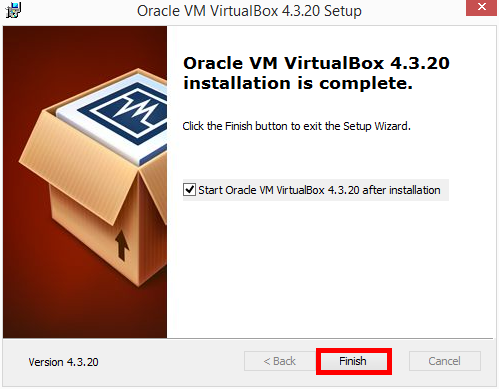
\includegraphics[width=0.49\columnwidth]{pictures/chapter3/vm6.png}
\end{figure}

\begin{figure}[h]
\centering
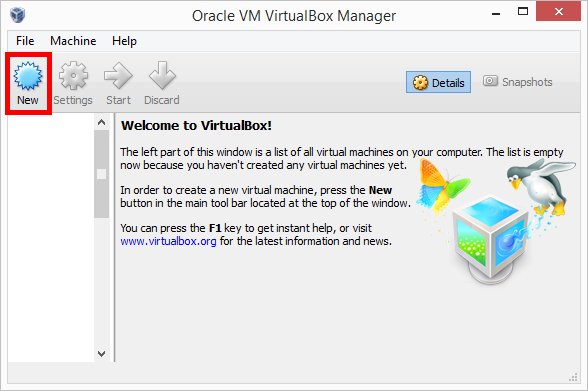
\includegraphics[width=0.49\columnwidth]{pictures/chapter3/vm7.png}
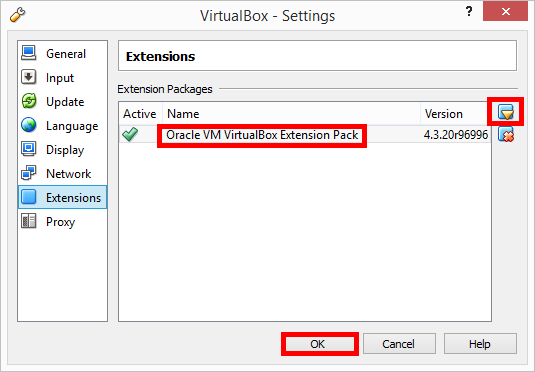
\includegraphics[width=0.49\columnwidth]{pictures/chapter3/vm8.png}
\end{figure}

\begin{figure}[h]
\centering
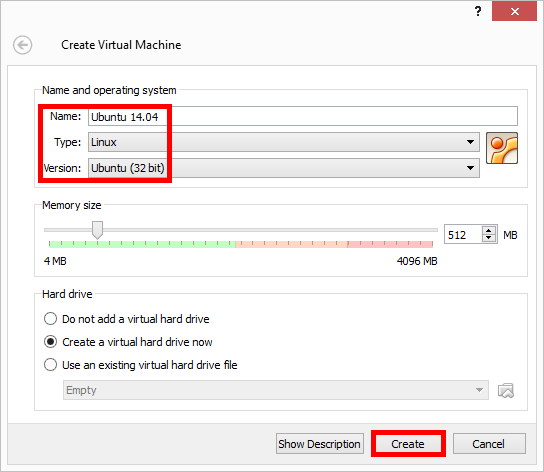
\includegraphics[width=0.49\columnwidth]{pictures/chapter3/vm9.png}
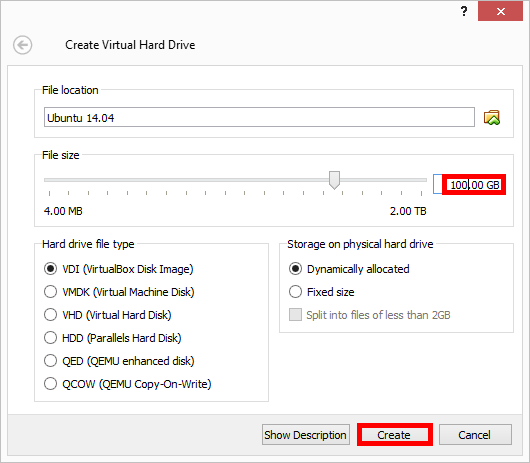
\includegraphics[width=0.49\columnwidth]{pictures/chapter3/vm10.png}
\end{figure}

\newpage

\begin{figure}[h]
\centering
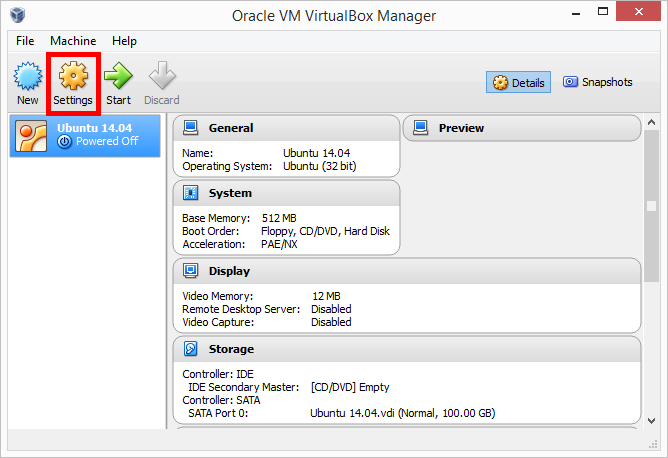
\includegraphics[width=0.49\columnwidth]{pictures/chapter3/vm11.png}
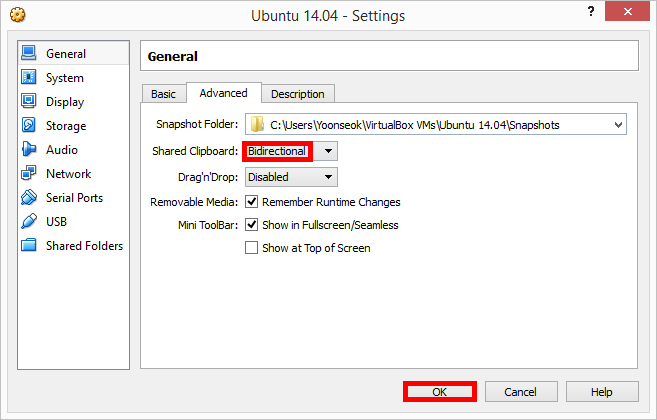
\includegraphics[width=0.49\columnwidth]{pictures/chapter3/vm12.png}
\end{figure}

\begin{figure}[h]
\centering
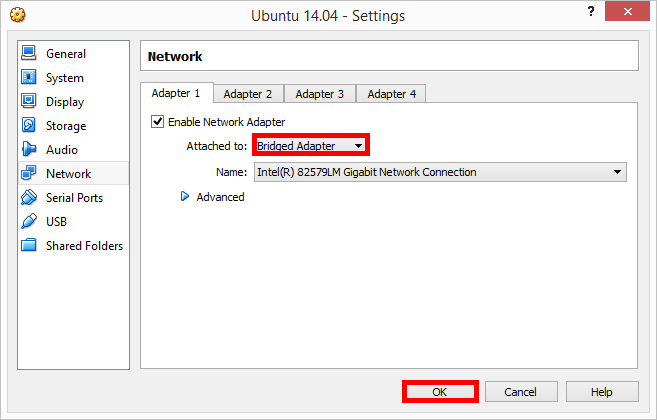
\includegraphics[width=0.49\columnwidth]{pictures/chapter3/vm13.png}
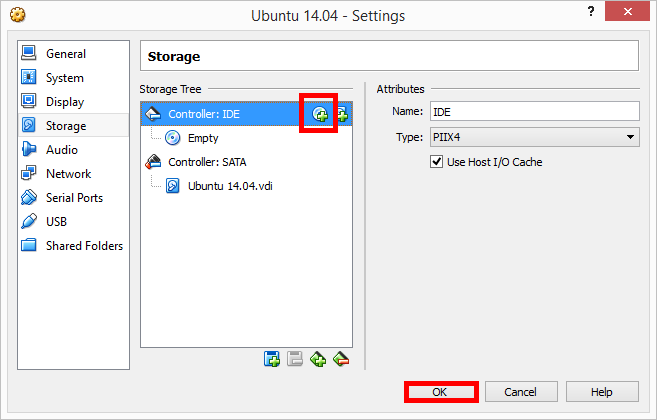
\includegraphics[width=0.49\columnwidth]{pictures/chapter3/vm14.png}
\end{figure}

\begin{figure}[h]
\centering
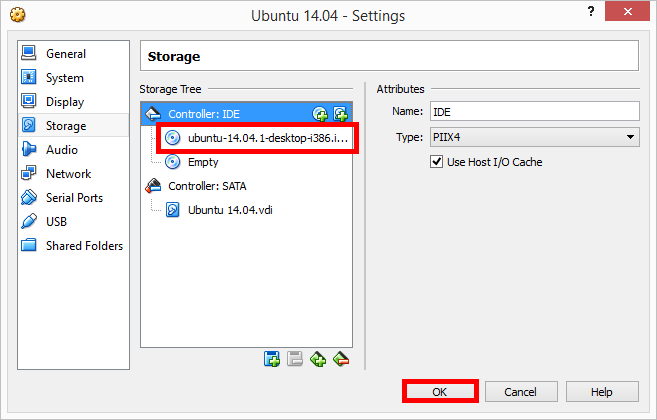
\includegraphics[width=0.49\columnwidth]{pictures/chapter3/vm15.png}
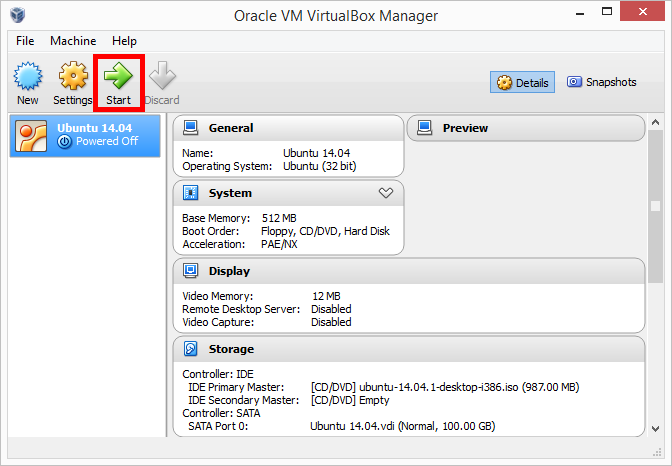
\includegraphics[width=0.49\columnwidth]{pictures/chapter3/vm16.png}
\end{figure}

\newpage

다음 그림들을 참고해가며 우분투를 설치하도록 하자. 우분투 설치가 마무리 되면 우분투 배포판이 나온 이후의 갱신에 대해서 다음의 명령어로 업데이트와 업그레이드를 해주도록 하자.

\begin{lstlisting}[language=ROS]
$ sudo apt-get update && sudo apt-get upgrade
\end{lstlisting}

\begin{figure}[h]
\centering
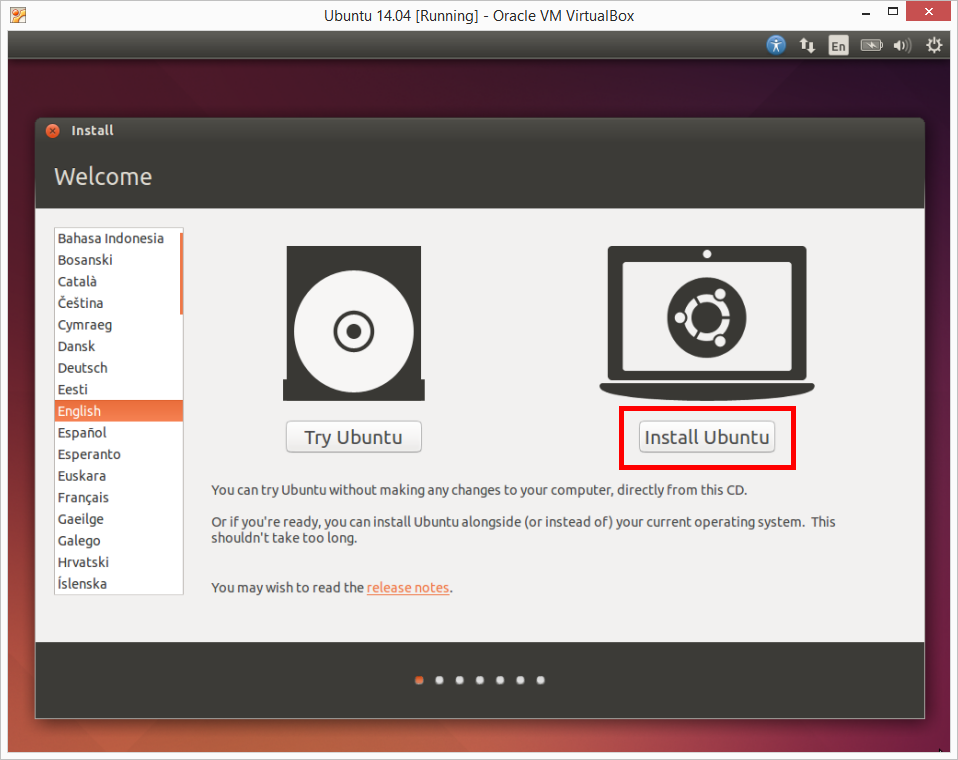
\includegraphics[width=0.45\columnwidth]{pictures/chapter3/vm17.png}
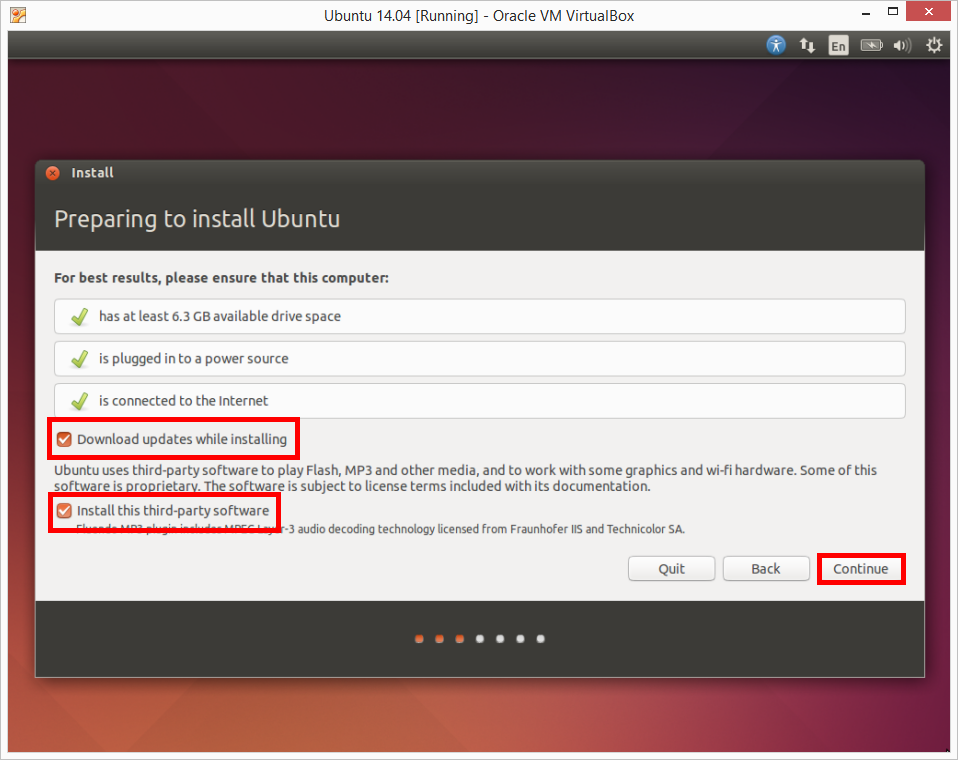
\includegraphics[width=0.45\columnwidth]{pictures/chapter3/vm18.png}
\end{figure}

\begin{figure}[h]
\centering
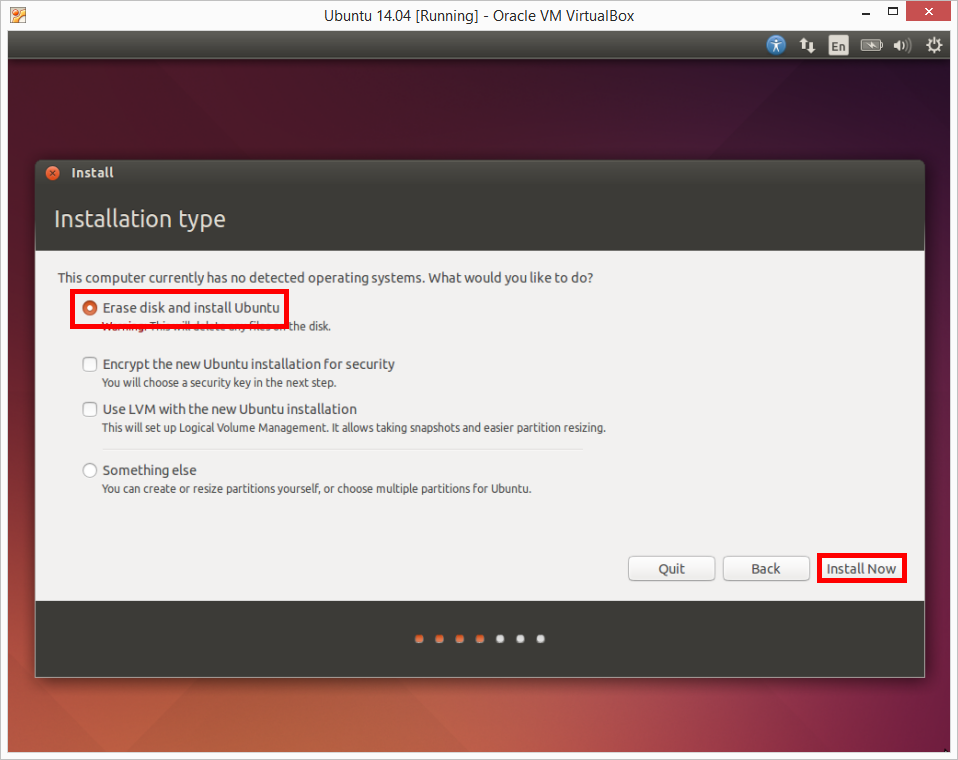
\includegraphics[width=0.45\columnwidth]{pictures/chapter3/vm19.png}
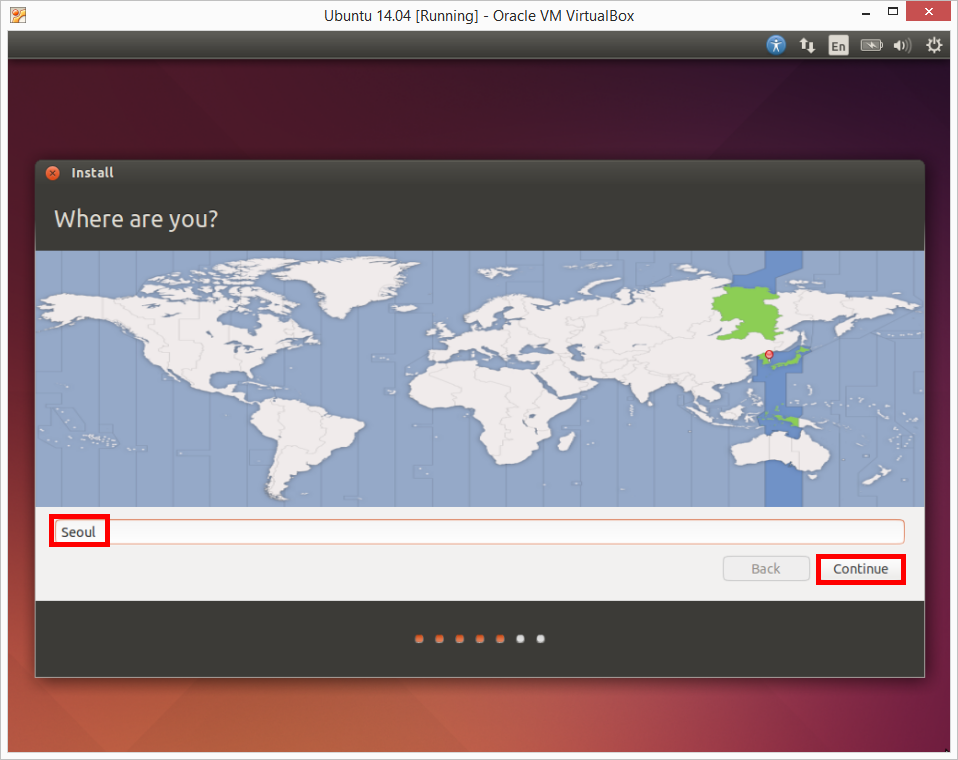
\includegraphics[width=0.45\columnwidth]{pictures/chapter3/vm20.png}
\end{figure}

\begin{figure}[h]
\centering
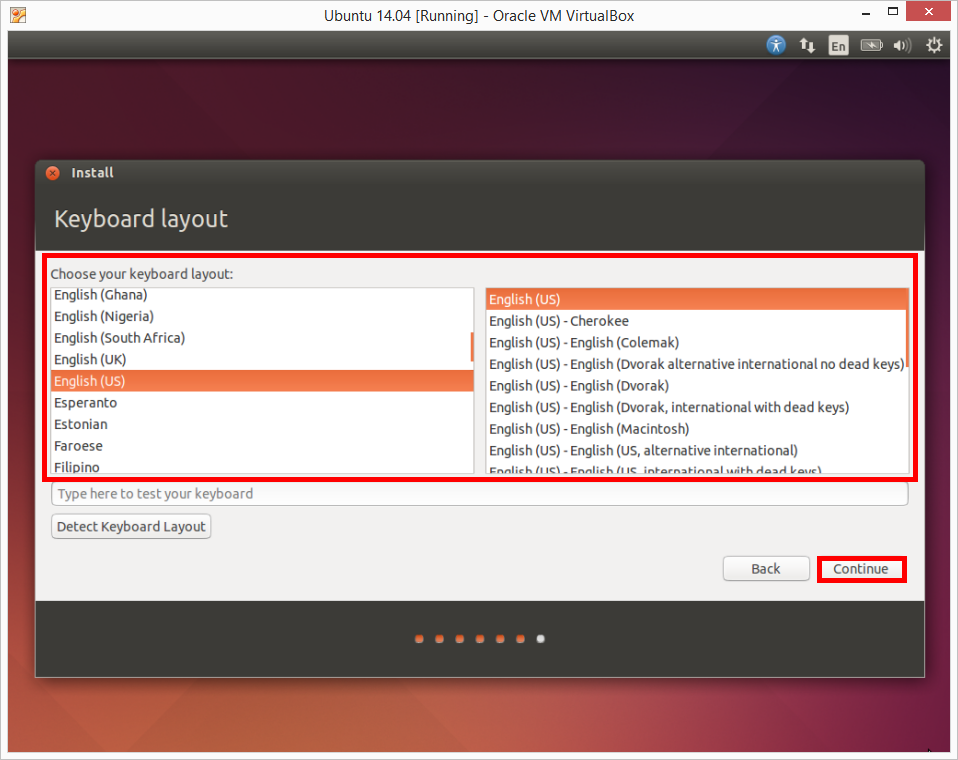
\includegraphics[width=0.45\columnwidth]{pictures/chapter3/vm21.png}
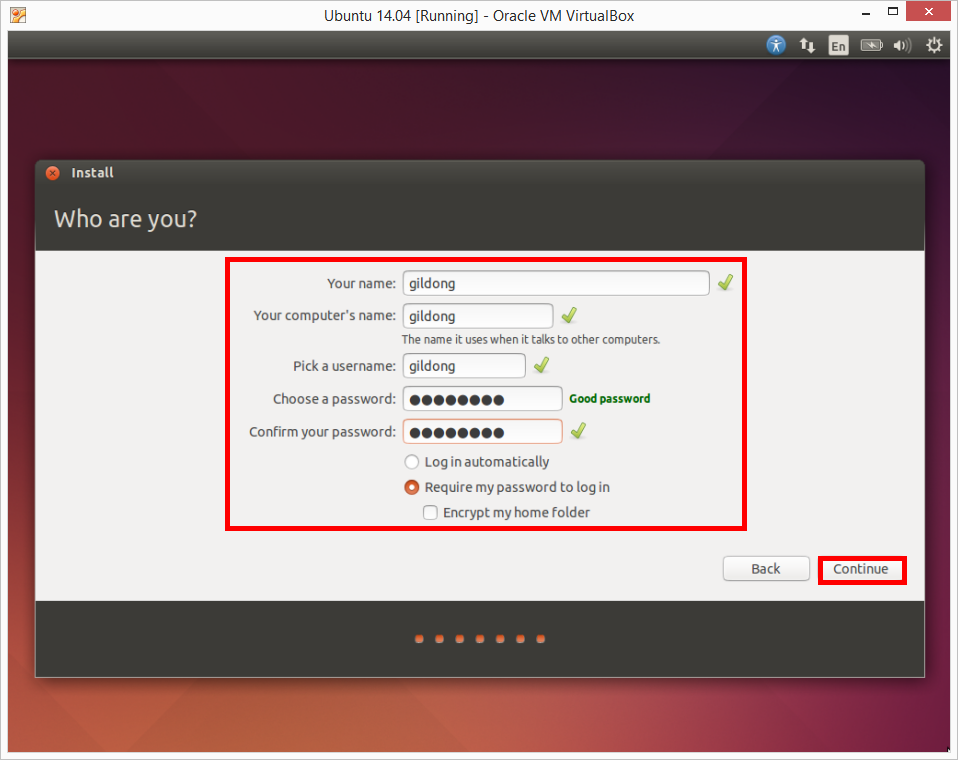
\includegraphics[width=0.45\columnwidth]{pictures/chapter3/vm22.png}
\end{figure}

\newpage

\begin{figure}[h]
\centering
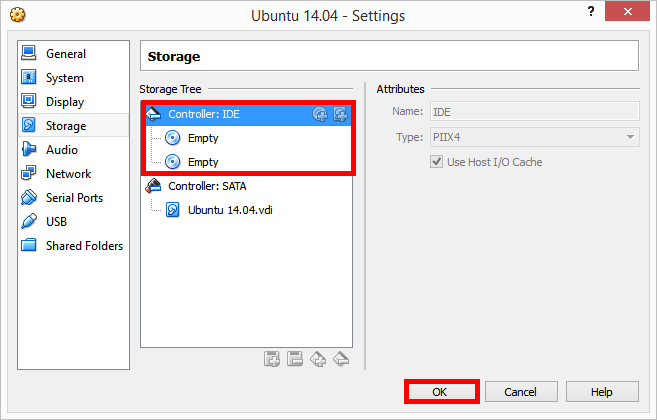
\includegraphics[width=0.49\columnwidth]{pictures/chapter3/vm23.png}
\end{figure}

%-------------------------------------------------------------------------------
\subsection{ROS Indigo 설치하기}\index{ROS Indigo 설치하기}

ROS Indigo 설치는 \textbf{섹션~\ref{sec:SimpleInstallation}}에서 설명한 간단 설치 방법으로 설치하도록 하겠다. 터미널 창을 열고 (Ctrl + Alt + t) 다음과 같이 간단 설치용 스크립트를 다운로드 한 후, 스크립트를 실행하여 ROS Indigo 설치하도록 하자.

\begin{lstlisting}[language=ROS]
$ wget https://raw.githubusercontent.com/oroca/oroca-ros-pkg/master/ros_indigo_install.sh
$ sh ros_indigo_install.sh
\end{lstlisting}

이제 모든 설치 작업이 완료되었다. 제대로 설치가 됐는지 알아보기 위하여 다음과 같이 roscore를 실행, 그리고 또 다른 새로운 터미널 창을 열고 turtlesim\_node를 구동하면 그림와 같이 실행될 것이다. 이 거북이를 보게 된다면 성공적으로 설치가 완료된 것이다.

\begin{lstlisting}[language=ROS]
$ roscore
$ rosrun turtlesim turtlesim_node
\end{lstlisting}

\begin{figure}[h]
\centering
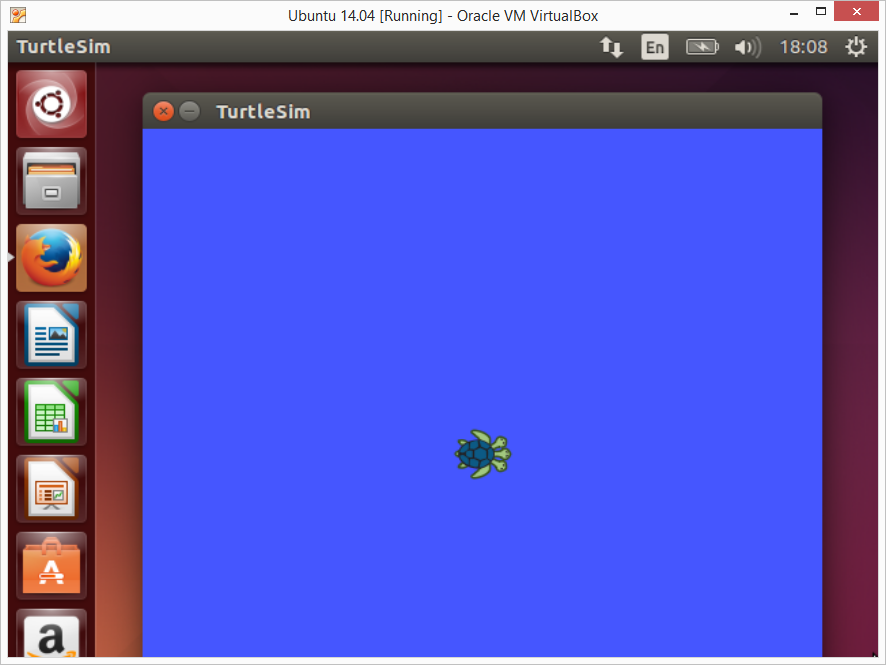
\includegraphics[width=0.49\columnwidth]{pictures/chapter3/vm24.png}
\end{figure}

%-------------------------------------------------------------------------------
\newpage
\section{라즈베리파이에 ROS Indigo 설치하기}\index{라즈베리파이에 ROS Indigo 설치하기}

%-------------------------------------------------------------------------------
\subsection{개발 환경}\index{개발 환경}

%-------------------------------------------------------------------------------
\subsection{ROS Indigo 설치하기}\index{ROS Indigo 설치하기}

% http://wiki.ros.org/ROSberryPi/Installing%20ROS%20Indigo%20on%20Raspberry%20Pi

%-------------------------------------------------------------------------------
\newpage
\section{오드로이드에 ROS Indigo 설치하기}\index{오드로이드에 ROS Indigo 설치하기}

\begin{figure}[h]
\centering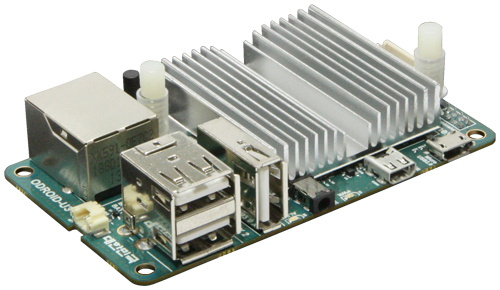
\includegraphics[width=0.5\columnwidth]{pictures/chapter3/odroid.jpg}
\caption{ODROID-U3}
\end{figure}

오픈소스 하드웨어 회사로 잘 알려진 국내 하드커널\footnote{\url{http://www.hardkernel.com/}}에서 개발한 오드로이드(ODROID-U3)는 ARM계열인 쿼드코어 1.7GHz Exynos 4412 Prime 를 사용하고 있어서 앞서 설명한 라즈베리파이 보다 월등한 성능 차이를 보이는 SBC의 한 종류이다. 더욱이 기본 OS로 루분투\footnote{\url{http://en.wikipedia.org/wiki/Lubuntu}}를 사용하고 있기에 우분투와 사용 방법은 비슷하면서도 LXDE\footnote{\url{http://ko.wikipedia.org/wiki/LXDE}} 데스크톱 환경을 사용하고 있어서 성능이 낮은 넷북, 휴대용 기기, 구형 PC에서도 매우 잘 돌아간다. 특히, 라즈베리파이에서는 영상 처리 혹은 Xtion, Kinect 같은 3차원 정보 취득에 있어서는 성능이 떨어지는 반면 오드로이드는 1.7GHz 쿼드코어와 2G RAM을 기본 탑재하고 있어서 사용함에 있어서 불편함이 없다.

오드로이드에 루분투를 설치하도록 하자. 오드로이드 우분투 자료실인 \url{http://odroid.in/ubuntu_14.04lts/} 에 접속하여 ubuntu-14.04.1lts-lubuntu-odroid-u-20141124.img.xz 을 다운로드 하자. 참고로 이 파일은 자주 갱신 되기 때문에 다운로드 받을시 언급한 버전이 아니더라도 ubuntu-14.04*으로 시작하는 가장 최신판을 다운로드 받으면 된다. 다운 받은 후 다음과 같이 압축을 해제하여 루분투의 ISO을 얻도록 하자.\\

\begin{lstlisting}[language=ROS]
$ xz -dv ubuntu-14.04.1lts-lubuntu-odroid-u-20141124.img.xz
\end{lstlisting}

다운로드한 이미지 파일을 SD 카드에 넣도록 하자. 완전 포맷되지 않은 SD 카드의 경우, 기존 파티션을 삭제 하도록 하자. 이를 위해서 우선 오드로이드가 아닌 데스크톱의 우분투에서 disks 를 시작 프로그램에서 선택하여 실행하자. 그 뒤 디스크 목록에서 해당 SD 카드를 선택하면 그림\ref{fig:partition_old} 좌측과 같이 기존 파티션들이 보일 것이다. 그 하단의 - 버튼을 클릭하여 기존 파티션을 모두 삭제하여 모든 영역을 Free Space로 만들면 그림\ref{fig:partition_old} 우측과 같은 결과를 얻을 수 있다.

\begin{figure}[h]
\centering
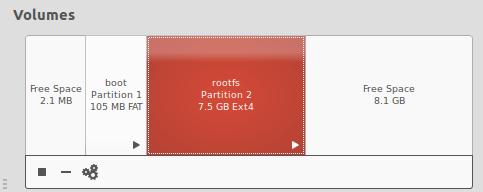
\includegraphics[width=0.45\columnwidth]{pictures/chapter3/odroid_partition1.png}
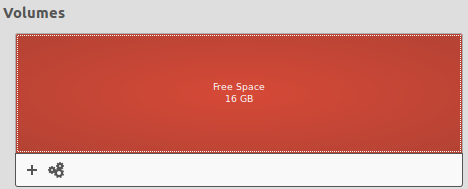
\includegraphics[width=0.44\columnwidth]{pictures/chapter3/odroid_partition2.png}
\caption{기존 파티션(좌)과 파티션 삭제(ㅇ)}
\label{fig:partition_old}
\end{figure}

그 다음 그림\ref{fig:partition_cleaned} 와 같은 disks 화면의 우측 상단의 버튼을 클릭하여 Restore disk image... 을 실행하자. 그림\ref{fig:open_img}처럼 imgae to Restore 의 파일 선택에서 이전 압축 해제한 이미지 파일을 선택하고 Start Restoring 를 클릭하면 10분 정도의 시간이 걸려 루분투 이미지가 리스토어 되게 된다. 리스토어가 완료되면 그림\ref{fig:partition_new} 과 같이 새로운 파티션들이 생성 되었음을 확인할 수 있다.

\begin{figure}[h]
\centering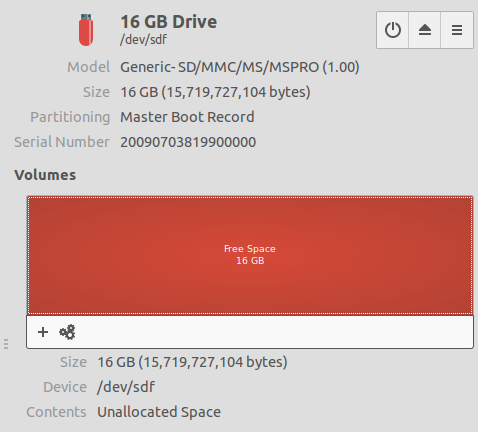
\includegraphics[width=0.5\columnwidth]{pictures/chapter3/odroid_sd.png}
\caption{디스크가 초기화된 상태}
\label{fig:partition_cleaned}
\end{figure}

\begin{figure}[h]
\centering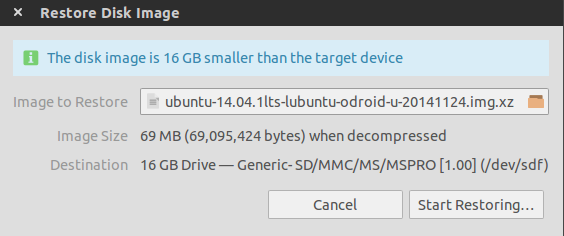
\includegraphics[width=0.49\columnwidth]{pictures/chapter3/odroid_restore.png}
\caption{리스토어 준비 과정}
\label{fig:open_img}
\end{figure}

\begin{figure}[h]
\centering
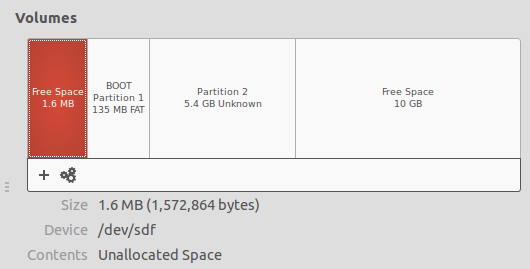
\includegraphics[width=0.5\columnwidth]{pictures/chapter3/odroid_partition3.png}
\caption{기존 파티션 삭제}
\label{fig:partition_new}
\end{figure}

리스토어한 SD 카드를 오드로이드에 삽입한 후, 전원을 넣고 부팅되면 그림\ref{fig:lxde}와 같이 루분투의 LXDE 데스크톱 환경을 볼 수 있다. 참고로 초기에는 로그인시 패스워드를 요구하지 않는다. 나중에 직접 패스워드를 지정해주도록 하자.

\begin{figure}[h]
\centering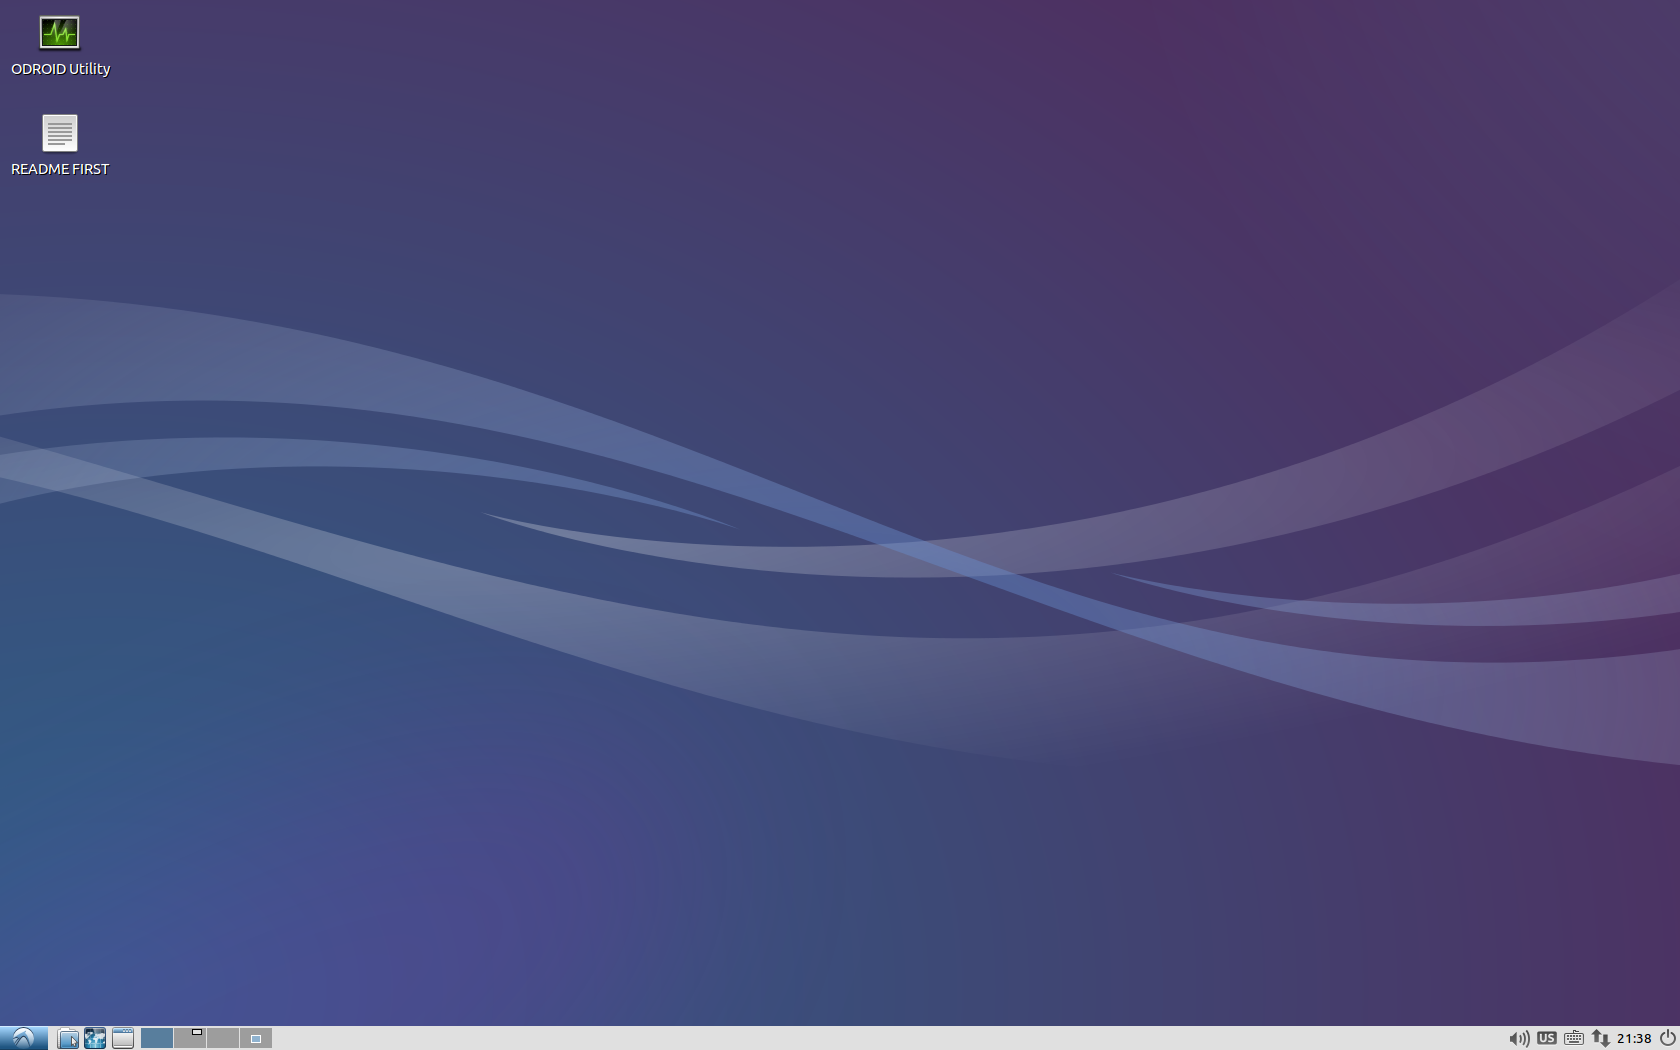
\includegraphics[width=0.5\columnwidth]{pictures/chapter3/odroid_LXDE.png}
\caption{LXDE 데스크톱}
\label{fig:lxde}
\end{figure}

우선, 현재 SD 메모리의 일부 부분만 사용할 수 있도록 되어 있기 때문에 메모리를 리사이즈 할 필요가 있다. LXDE 화면 하단의 xterm 을 실행하여 다음과 같이 오드로이드 유틸리티를 실행하자. 그 후 그림\ref{fig:odroid_utility}와 같이 메모리 리사이즈를 하기 위하여 4.Resize your root partition 를 선택하여 리사이징을 해주자.

\begin{lstlisting}[language=ROS]
$ sudo  odroid-utility.sh 
\end{lstlisting}

\begin{figure}[h]
\centering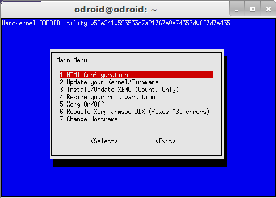
\includegraphics[width=0.5\columnwidth]{pictures/chapter3/odroid_option1.png}
\caption{오드로이드 유틸리티 화면}
\label{fig:odroid_utility}
\end{figure}

\begin{figure}[h]
\centering
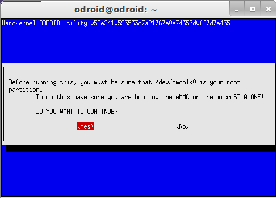
\includegraphics[width=0.4\columnwidth]{pictures/chapter3/odroid_option2.png}
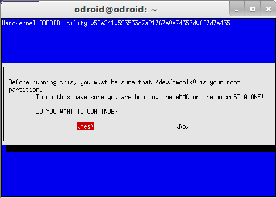
\includegraphics[width=0.4\columnwidth]{pictures/chapter3/odroid_option3.png}
\caption{리사이징 과정}
\end{figure}

\newpage

리사이징이 완료되었으며 아래와 같이 재부팅을 하자.

\begin{lstlisting}[language=ROS]
$ sudo reboot 
\end{lstlisting}

그다음 다음의 명령어로 ROS Indigo를 설치하자.

\begin{lstlisting}[language=ROS]
$ sudo update-locale LANG=C LANGUAGE=C LC_ALL=C LC_MESSAGES=POSIX
$ sudo sh -c 'echo "deb http://packages.namniart.com/repos/ros trusty main" > /etc/apt/sources.list.d/ros-latest.list'
$ wget http://packages.namniart.com/repos/namniart.key -O - | sudo apt-key add -
$ sudo apt-get update
$ sudo apt-get install ros-indigo-ros-base
$ sudo apt-get install python-rosdep
$ sudo rosdep init
$ rosdep update
$ echo "source /opt/ros/indigo/setup.bash" >> ~/.bashrc
$ source ~/.bashrc
$ sudo apt-get install python-rosinstall
\end{lstlisting}

다음에는 다음과 같이 catkin work space 폴더를 만들고 catkin\_make 가 정상 작동하는지 살펴보자.

\begin{lstlisting}[language=ROS]
$ source /opt/ros/indigo/setup.bash
$ mkdir -p ~/catkin_ws/src
$ cd ~/catkin_ws/src
$ catkin_init_workspace
$ cd ~/catkin_ws/
$ catkin_make
\end{lstlisting}

마지막으로 roscore 가 동작하는지 테스트하면 모든 설치가 완료된 것이다.

\begin{lstlisting}[language=ROS]
$ roscore
\end{lstlisting}

%-------------------------------------------------------------------------------


































































%-------------------------------------------------------------------------------